
% ----------------------------------------------------------------------
%  Set the document class
% ----------------------------------------------------------------------
\documentclass[11pt,a4paper,twoside]{article}

% ----------------------------------------------------------------------
% Define external packages, language, margins, fonts and new commands
% ----------------------------------------------------------------------
%\input{preamble} 
\usepackage[utf8]{inputenc}   % <<<<< Linux
\usepackage[english]{babel} % <<<<< English
\usepackage{notoccite}
\usepackage[skip=0.5\baselineskip]{caption}
\hyphenation{GTKWave}
\usepackage{listings}
\usepackage[all]{nowidow}

\usepackage{systeme}
  % tables
\usepackage{multirow}
\usepackage{tabularx}
\usepackage{booktabs}
\usepackage{supertabular}


%blind text
\usepackage{lipsum}

\usepackage{comment} % comment out large bodies of text

\usepackage{graphicx}
\graphicspath{ {./} {../../figlib/} }
\def\FontLn{% 16 pt normal
  \usefont{T1}{phv}{m}{n}\fontsize{16pt}{16pt}\selectfont}
\def\FontLb{% 16 pt bold
  \usefont{T1}{phv}{b}{n}\fontsize{16pt}{16pt}\selectfont}
\def\FontMn{% 14 pt normal
  \usefont{T1}{phv}{m}{n}\fontsize{14pt}{14pt}\selectfont}
\def\FontMb{% 14 pt bold
  \usefont{T1}{phv}{b}{n}\fontsize{14pt}{14pt}\selectfont}
\def\FontSn{% 12 pt normal
  \usefont{T1}{phv}{m}{n}\fontsize{12pt}{12pt}\selectfont}

% Use Arial font as default
%
\renewcommand{\rmdefault}{phv}
\renewcommand{\sfdefault}{phv}
\usepackage{geometry}	
\geometry{verbose,tmargin=2.5cm,bmargin=2.5cm,lmargin=2.5cm,rmargin=2.5cm}

%\usepackage{setspace}
%\renewcommand{\baselinestretch}{1.5}

\usepackage[pdftex]{hyperref} % enhance documents that are to be
                              % output as HTML and PDF
\hypersetup{colorlinks,       % color text of links and anchors,
                              % eliminates borders around links
%            linkcolor=red,    % color for normal internal links
            linkcolor=black,  % color for normal internal links
            anchorcolor=black,% color for anchor text
%            citecolor=green,  % color for bibliographical citations
            citecolor=black,  % color for bibliographical citations
%            filecolor=magenta,% color for URLs which open local files
            filecolor=black,  % color for URLs which open local files
%            menucolor=red,    % color for Acrobat menu items
            menucolor=black,  % color for Acrobat menu items
%            pagecolor=red,    % color for links to other pages
            pagecolor=black,  % color for links to other pages
%            urlcolor=cyan,    % color for linked URLs
            urlcolor=black,   % color for linked URLs
	          bookmarks=true,         % create PDF bookmarks
	          bookmarksopen=false,    % don't expand bookmarks
	          bookmarksnumbered=true, % number bookmarks
	          pdftitle={report},
            pdfauthor={Conanga, H.P.},
%            pdfsubject={Thesis Title},
%            pdfkeywords={Thesis Keywords},
            pdfstartview=FitV,
            pdfdisplaydoctitle=true}

\usepackage[numbers,sort&compress]{natbib} % <<<<< References in numbered list [1],[2],...
\usepackage{subcaption} 
\usepackage{mdframed}
\usepackage{amsmath} % facilitates writing math formulas and improves the typographical quality of their output
\usepackage{siunitx} % facilitates writing SI units, along with other SI unit related features
\setcounter{MaxMatrixCols}{20} % enables latex to make matrices w/ 20 columns
\usepackage{float} % not sure


%%%%%%%%%%%%%%%%%%%%%%%%%%%%%%%%%%%%%%%%%%%%%%%%%%%%%%%%%%%%%%%%%%%%%%%%
%     Begin Document                                                   %
%%%%%%%%%%%%%%%%%%%%%%%%%%%%%%%%%%%%%%%%%%%%%%%%%%%%%%%%%%%%%%%%%%%%%%%%


\begin{document}

% Set plain page style (no headers, footer with centered page number)
\pagestyle{plain}

% Set roman numbering (i,ii,...) before the start of chapters
%\pagenumbering{roman}

% ----------------------------------------------------------------------
%  Cover page
% ----------------------------------------------------------------------
%%%%%%%%%%%%%%%%%%%%%%%%%%%%%%%%%%%%%%%%%%%%%%%%%%%%%%%%%%%%%%%%%%%%%%%%
%                                                                      %
%     File: Thesis_FrontCover.tex                                      %
%     Tex Master: Thesis.tex                                           %
%                                                                      %
%     Author: Andre C. Marta                                           %
%     Last modified :  2 Jul 2015                                      %
%                                                                      %
%%%%%%%%%%%%%%%%%%%%%%%%%%%%%%%%%%%%%%%%%%%%%%%%%%%%%%%%%%%%%%%%%%%%%%%%

\thispagestyle {empty}

% IST Logo - Signature A
% parameters: bb=llx lly urx ury (bounding box), width=h_length, height=v_length, angle=angle, scale=factor, clip=true/false, draft=true/false. 
%\includegraphics[bb=9.5cm 11cm 0cm 0cm,scale=0.29]{IST_A_CMYK_POS}

\begin{center}
%
% Figure (Image or plot)
\vspace{1.0cm}
% height = 50 mm
%\includegraphics[height=50mm]{Figures/Airbus_A350.jpg}

% Title, author and degree
\vspace{1cm}
{\FontLb Circuit Theory and Electronics Fundamentals} \\ % <<<<< EDIT TITLE
\vspace{1cm}
{\FontSn BSc Aerospace Engineering, Técnico, University of Lisbon} \\ % <<<<< EDIT COURSE
\vspace{1cm}
{\FontSn Lab 1: Circuit analysis methods} \\
\vspace{1cm}
{\FontSn March 25, 2021} \\ % <<<<< EDIT DATE (corresponds to date of oral examination)
\vspace{1cm}
{\FontSn Group 48} \\ %group
{\FontSn Dinis Papinha, 84379} \\ %authors
{\FontSn Filipa Gonçalves, 89662} \\ %authors
{\FontSn Carlos de Vasconcelos, 90227} \\ %authors
%
\end{center}


% ----------------------------------------------------------------------
% Dedication page (optional)
% ----------------------------------------------------------------------
%\input{dedication} 
%\cleardoublepage

% ----------------------------------------------------------------------
%  Acknowledgments (optional)
% ----------------------------------------------------------------------
%\input{acknowledgements}
%\cleardoublepage

% ----------------------------------------------------------------------
%  Abstract (both in English and Portuguese)
% ----------------------------------------------------------------------
%\input{resumo} 
%\cleardoublepage

%\input{abstract} 

% ----------------------------------------------------------------------
%  Table of contents, list of tables, list of figures and nomenclature
% ----------------------------------------------------------------------

% Table of contents
%
\tableofcontents

% List of tables
%\addcontentsline{toc}{section}{\listtablename}
%\listoftables
%\cleardoublepage 

% List of figures
%\addcontentsline{toc}{section}{\listfigurename}
%\listoffigures
%\cleardoublepage 

% Set arabic numbering (1,2,...) after preface
%
%\setcounter{page}{1}
%\pagenumbering{arabic}

% ----------------------------------------------------------------------
%  Body
% ----------------------------------------------------------------------

\section{Introduction}
\label{sec:introduction}

% state the learning objective 
The objective of this laboratory assignment is to study a RC circuit containing linear components, 
such as resistors ($R_i$), dependent (rhombus shaped) voltage ($V$) and current ($I$) 
sources, a capacitor $C$ and a an independent (circle shaped) voltage source, as seen in Figure~\ref{fig:OG_circ}, in which the nodes are ilustrated and the functions that define the sources are presented.


In Section~\ref{sec:analysis}, a theoretical analysis of the circuit is
presented, using the \textit{Octave}. This analysis includes determining the currents through the branches and the voltages in the nodes for $t<0$, obtaining the equivalent resistance as seen from the capacitor terminals, determining the natural and forced solutions and superimposing them to determine the total solution for $t>0$, and performing a frequency analysis. 
In Section~\ref{sec:simulation}, an analogous analysis is made through simulation, using \textit{Ngspice}, and the results are compared to the theoretical results obtained in Section~\ref{sec:analysis}. The conclusions of this study are outlined in
Section~\ref{sec:conclusion}.


\begin{figure}[h] \centering
    \includegraphics[width=0.8\linewidth]{original_circuit.pdf}
    \caption{Original RC circuit.}
    \label{fig:OG_circ}
    \end{figure}
    





\newpage
\section{Theoretical Analysis}
\label{sec:analysis}

To make this analysis we used the following parameters values (of the circuit components that could be manipulated):


\begin{table}[h]
\centering
\begin{tabular}{ll}

Co & 1e-6 \\
Ci=Cb & 1e-3 \\
R1 & 80k \\
R2 & 20k  \\
RC & 1000 \\
RE & 100 
\end{tabular}
\end{table}

Hence the overall cost of the architecture is 1102.4 MU.

Considering the analyzed circuit, it is understood that the first stage is responsible for the amplication of the signal so that it is not degradated along the circuit. As such it is expected for it to have a high gain. 
Solving the OP problem with the help of Octave it is possible to obtaine $VCE=2.1578$

Regarding the gains plots between the first and 2 stage we can see that they do not differ alot, this is beliveble since AV2=-0.0348 db as we can see in the table, so it does not vary much the result.


\begin{figure}[h]
\centering
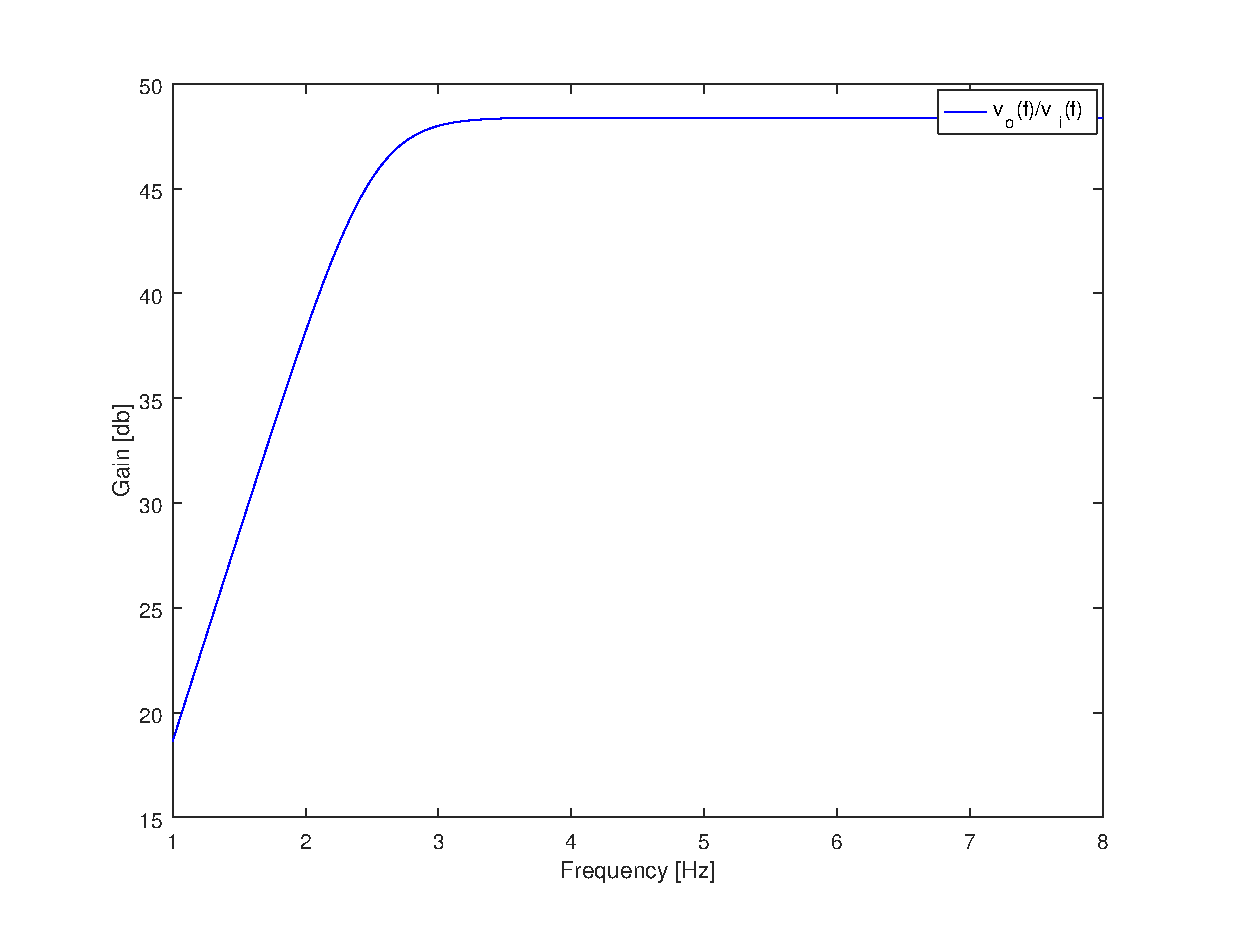
\includegraphics[width=0.6\linewidth]{Gain1.eps}
\caption{Gain in the first phase}
\label{plot:ganho1}
\end{figure}

\newpage

Nevertheless the inputs and outputs for this stages are present in the following table:

\begin{table}[h]
\centering
\begin{tabular}{ll}

AV1 & 48.39 \\
ZI1 & 484.43 \\
Z01 & 886.28 \\
AV2 & -0.0348  \\
ZI2 & 8598.9 \\
Z02 & 0.302 
\end{tabular}
\end{table}

\newpage

As we can see in the previous table, after the first stage the output impedance ($Z01$) increases. To contrariate that, it is added a new stage that decreases the output impedance. As a consequece we can connect this stages without a significant signal loss. Important to note that $AV2=0.996$, 
because it has a value near 1, this leads to small amplifications or attenuations
As such the final gain plot can be given by the following Figure.
\begin{figure}[h]
\centering
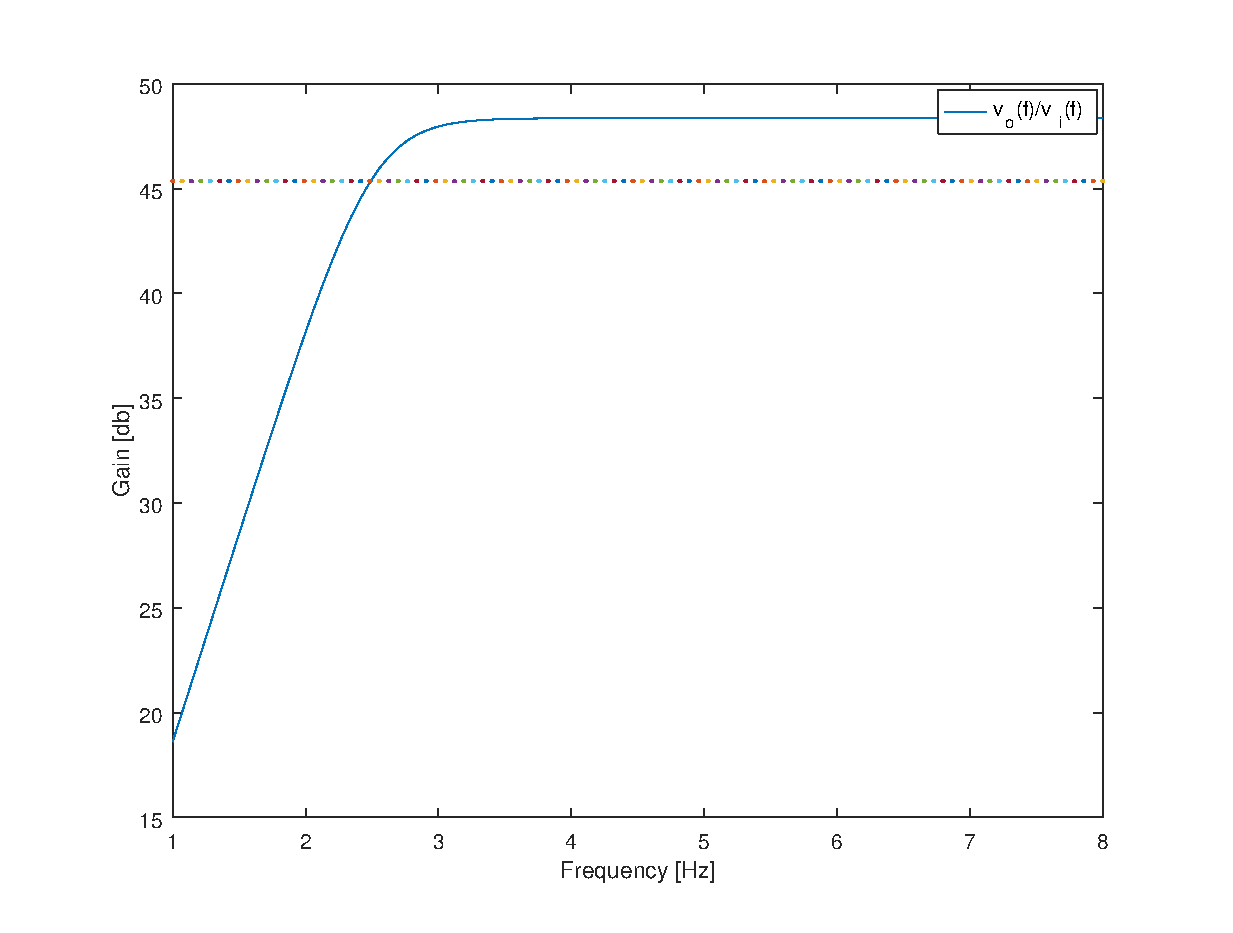
\includegraphics[width=0.6\linewidth]{GainFinal.eps}
\caption{Output Gain}
\label{plot:ganho2}
\end{figure}

Analyzing these plots we can see that they are high pass filter. Because it was expected a band pass an incorrect analsis of the circuit was most certainly made.

\section{Simulation Analysis}
\label{sec:simulation}

In this section, the intent is to simulate the circuit, using \textit{Ngspice} software with the model uA741 as the AMP-OP.

Time and, more importantly, frequency analysis were performed in order to evaluate the circuit in the passband (specifically, the output voltage gain along with its phase), the central frequency of the passband, and the input (Zin) and output (Zout) impedances in the central frequency. The following table represents the major results of interest.

\begin{table}[h]
    \centering
    \begin{tabular}{|l|r|}
      \hline    
      {\bf Name} & {\bf Value [A or V]} \\ \hline
      \input{../doc/op_results_tab.tex}
      \input{../doc/op_Zin_tab.tex}
      \input{../doc/op_Zout_tab.tex}
    \end{tabular}
    \caption{Main results measured in NGSpice software.}
 \end{table}

Note that the gain at 1kHz isn't in dBs, but in volts: it corresponds to 42.02628 dBs.
The following figures are the computations of the output voltage gain and its phase as a function of frequency.

\begin{figure}[!htb]
    \centering
    \includegraphics[width=0.9\textwidth]{../doc/vdbo2f.pdf}
    \caption{\textit{Ngspice's} output voltage gain}
\end{figure}

\begin{figure}[!htb]
    \centering
    \includegraphics[width=0.9\textwidth]{../doc/vpho2f.pdf}
    \caption{Phase frequency analysis of the output voltage gain using NGSpice.}
\end{figure}



\clearpage

\subsection{Comparasion}
\label{sec:comparasion}

Here, the results obtained with each software / approach are presented.




The obtained obtained values in the tables are approximatly the same and in the plots aswell. The differences in the gain plots are present mostly at higher frequencies, after the peak, which occurs at about 1kHz and 40dBs in both analysis, as intended. After those frequencies, and namely around 10kHz, the gain obtained with Ngspice drops a lot faster. The aformentioned discrepancies may be due to the fact that Ngpice uses models a lot more complex than the ones considered in our theoretical analysis. Specifically, the said increase in complexity and exactitude (with Ngspice) may lead to a greater effect of the input impedance drop at higher frequencies, that may naturally result in a greater drop in the output voltage gain. The differences in the phase plots also come from the greater complexity in the models used by the Ngspice software. Ngspice performs the simulation considering that the AMP-OP has two capacitors and, in the theoretical analysis, they are disregarded. As such, the Ngspice plot predicts a decrease of an extra 180 degrees (-90 degrees for each capacitor), which is not expected in the Octave plot.

Note that, considering both the simulation and the theoretical analysis approach, the circuit does function like a passband circuit, with a narrow yet significant bandwith, centered around the frequency and gain established as goals. as seen in the presented figures.

\section{Conclusion}
\label{sec:conclusion}

In this laboratory assignment the objective of analysing an RC circuit has been
achieved. Static, time and frequency analyses have been performed both
theoretically using the Octave maths tool and by circuit simulation using the
Ngspice tool. The simulation results matched the theoretical results
precisely. The reason for this perfect match is the fact that this is a
straightforward circuit containing only linear components, so the theoretical


%\cleardoublepage

% ----------------------------------------------------------------------
%  Bibliography
% ----------------------------------------------------------------------
%\addcontentsline{toc}{section}{\bibname}
%\bibliographystyle{abbrvunsrtnat} % <<<<< SELECT IF USING REFERENCES BY NUMBER (CITATION ORDER)
%\bibliography{../../../BIBfile.bib}

% ----------------------------------------------------------------------
\end{document}
% ----------------------------------------------------------------------

